%第2章:準備
%システムを開発する際,使用した定義.


本章では,研究方針のフローと,本論文で使用する用語について述べる.

\subsection*{V字モデル[5]}

V字モデルとはソフトウェアの開発と確認の流れを模式的に示したものである.以下の図\ref{vji}にV字モデルの開発プロセスを示す.横軸は開発の時間軸であり,縦軸は詳細化の程度を表している\cite{kumikomi}.図\ref{vji}にも示すように,詳細設計は単体テスト,基本設計は結合テストによって,要求分析は総合テストによって検証する.また,逆にテスト段階で判明した不具合は,左側の対応する設計にさかのぼった作業を必要とする.本研究では開発プロセスモデルとしてV字モデルを採用した.

\begin{figure}[htbp]
\centering
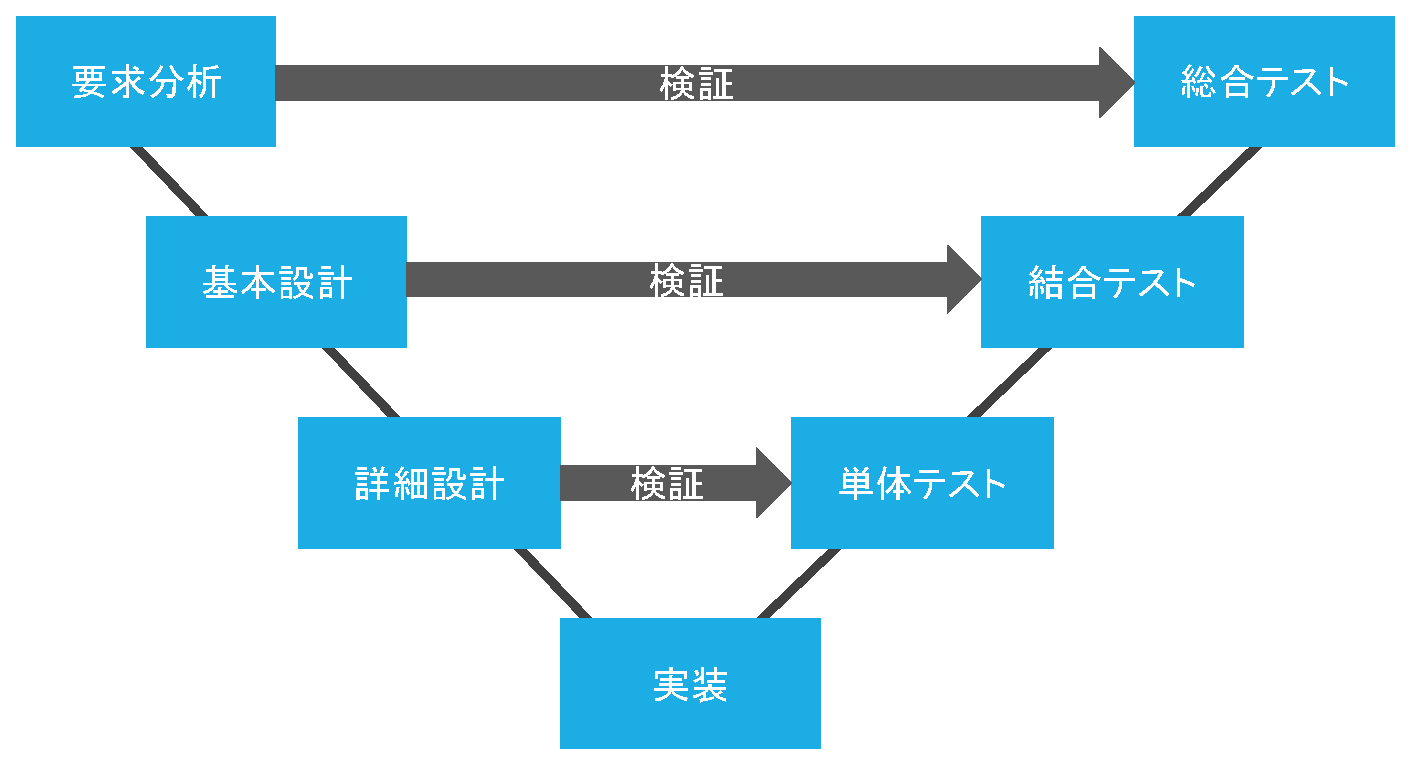
\includegraphics[width=12cm]{./picture/vjimodel.eps}
\caption{V字モデル}
\label{vji}
\end{figure}


\subsection*{UML(Unifiled Modeling Language)[3]}

UMLとは統一モデリング言語(Unified Modeling Language)のことで,ビジネスや各種システムを対象としてその構造とダイナミクス(動的な振る舞いや挙動)をわかりやすく表現するためのビジュアルな言語である\cite{uml}.UMLの導入により,下記のような効用がもたらされる.

\begin{itemize}
\item ユーザと開発者,または開発者どうしのコミュニケーションギャップの解消.
\item ユーザ要求の把握が正確になることで,仕様の認識違いによる出戻りの削減.
\item UMLによるオブジェクト指向設計が効果的にモジュール化を促進し,保守コストを削減.
\end{itemize}

\subsection*{ユースケース図[3]}

ユースケース図とは,UMLで定義されている図のうちのひとつである.ユーザの視点でシステムの機能的な流れを記述する記述法\cite{soft}であり,システムの使用イメージを表現する.システムがどのように機能すべきかという振る舞い(ユースケース)と,その外部環境(アクター)を表す.ユーザやクライアントの要求事項,システムに対して課せられている基本機能やサービス項目などの要件定義を表現するときに広く用いられる.

\subsection*{クラス図[3]}

クラス図はUMLの基本となる図のひとつである.システムをデータの視点から記述する図法\cite{soft}であり,システムが扱う情報構造を表す.問題領域の構造や対象システムの静的な構成,システムの詳細設計,あるいは企業の部門の業務モデルの基本構造,問題解決の最初のとっかかりとなる概念マップの構築,といったことに広く使うことができる.

\subsection*{シーケンス図[3]}

シーケンス図とは,UMLで定義されている相互作用図の一種類である.システムの一機能を実行の視点から記述する図法\cite{soft}	であり,システム機能がオブジェクトのメッセージのやり取りによってどのように達成されるかを示す.オブジェクト間のメッセージのやりとりを時系列に沿って並べて表現したものがシーケンス図である.